\documentclass[xcolor={dvipsnames}]{beamer}

\usetheme{Copenhagen}

\setbeamertemplate{itemize items}[default]
\setbeamertemplate{enumerate items}[default]

\setbeamercolor*{structure}{bg=PineGreen!20, fg=PineGreen}

\setbeamercolor*{palette primary}{use=structure, fg=white, bg=structure.fg}
\setbeamercolor*{palette secondary}{use=structure, fg=white, bg=structure.fg!75}
\setbeamercolor*{palette tertiary}{use=structure, fg=white, bg=structure.fg!75}
\setbeamercolor*{palette quaternary}{use=structure, fg=white, bg=structure.fg!75}

\setbeamercolor{section in toc}{fg=black, bg=white}
\setbeamercolor{alterted text}{use=structure, fg=structure.bg!50!black!80!black}

\setbeamercolor{titlelike}{parent=palette primary, fg=structure.fg!50!black}
\setbeamercolor{frametitle}{bg=gray!10!white, fg=PineGreen}

\setbeamercolor*{titlelike}{parent=palette primary}

\usepackage{amsmath}

\usepackage{algorithm2e}

\usepackage{graphicx}

\usepackage{tikz}
\usepackage{tikzducks}
\usetikzlibrary{arrows, shapes, positioning, fit, ducks}

\title{Introduction to Machine Learning}
\subtitle{Sample Lecture and Lab}
\date{}
\author{Computer Science}
\institute{}

\begin{document}

\frame{\titlepage}

\begin{frame}
	\frametitle{Purpose}

	\begin{itemize}
		\item{Understand machine learning}
			\begin{itemize}
				\item{Basic concepts}
				\item{Working with data}
				\item{\(k\) nearest neighbours}
				\item{Neural networks/multilayer perceptrons}
				\item{Measuring performance}
			\end{itemize}
		\item{Learn about studying at university}
	\end{itemize}
\end{frame}

\begin{frame}
	\frametitle{Session Structure}

	\begin{figure}
		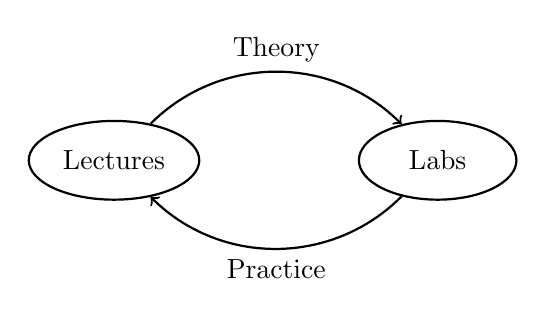
\begin{tikzpicture}[node distance=2cm]
			\node [draw, ellipse, thick, minimum height=1cm,
			minimum width=2cm]
			(lectures) {Lectures};
		
			\node [right=of lectures, draw, ellipse, thick, minimum
			height=1cm, minimum width=2cm] (labs) {Labs};

			\draw [thick, ->]
				(lectures) edge [bend left=45] node [above] {Theory} (labs)
				(labs) edge [bend left=45] node [below] {Practice} (lectures);
		\end{tikzpicture}
	\end{figure}

	\begin{itemize}
		\item{50\% lecture - exploring machine learning}
		\item{50\% lab - applying ML techniques to a dataset}
	\end{itemize}
\end{frame}

\begin{frame}
	\frametitle{What is Machine Learning?}

	Getting computers to find patterns in data \textbf{without actually
	telling it what to look for!}

	\begin{figure}
		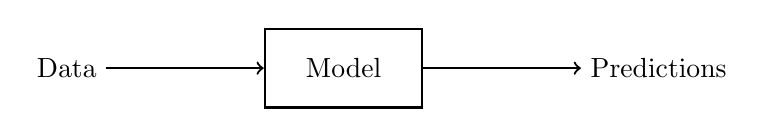
\begin{tikzpicture}[node distance=2cm]
			\node (data) {Data};
			\node (model) [right=of data, draw, rectangle, thick,
			minimum height=1cm, minimum width=2cm] {Model};
			\node (predictions) [right=of model] {Predictions};

			\draw [thick, ->] (data) -- (model);
			\draw [thick, ->] (model) -- (predictions);
		\end{tikzpicture}
	\end{figure}

	Consists of feeding some \textit{training data} to a computer to 
	create a \textit{model} which can make \textit{predictions}.

	\begin{itemize}
		\item{Predictions can be on new/unseen data}
		\item{Predictions can be about data itself}
		\item{Predictions can be next action to take}
	\end{itemize}
\end{frame}

\begin{frame}
	\frametitle{Why use Machine Learning?}

	\begin{figure}
		\begin{tikzpicture}[node distance=1cm]
			\node (mnist)
			{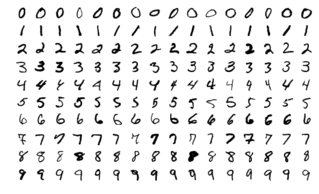
\includegraphics[width=0.5\textwidth]{img/mnist-example.png}};
			
			\node (question) [right=of mnist] {?};

			\draw [thick, ->] (mnist) -- (question);
		\end{tikzpicture}
	\end{figure}

	Some problems are difficult to solve using conventional algorithms. For
	these, it is better to let machines find their own solutions instead of
	manually specifying how to solve them manually.
\end{frame}

\begin{frame}
	\frametitle{Types of Machine Learning Problems}

	\begin{figure}
		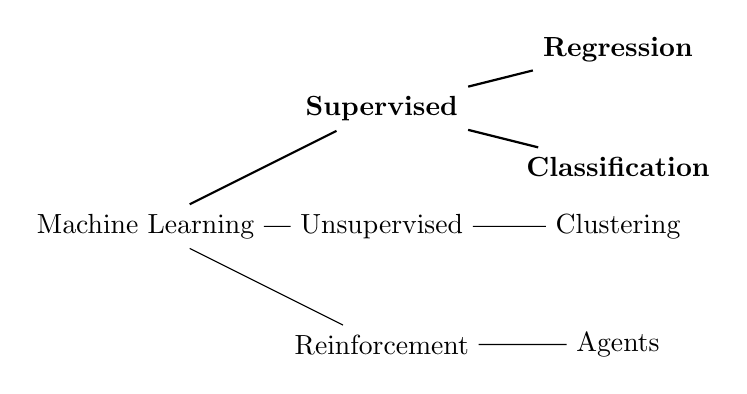
\begin{tikzpicture}[level distance=3cm]
			\node (tree) {Machine Learning} [grow'=right]
			child [thick] {node {\textbf{Supervised}}
				child {node {\textbf{Regression}}}
				child {node {\textbf{Classification}}}}
			child {node {Unsupervised}
				child {node {Clustering}}}
			child {node {Reinforcement}
				child {node {Agents}}};
		\end{tikzpicture}
	\end{figure}

	\begin{itemize}
		\item{Supervised learning: using data with labelled outcomes}
			\begin{itemize}
				\item{Regression: predicting a continuous
					value}
				\item{Classification: predicting a discrete
					value}
			\end{itemize}
	\end{itemize}
\end{frame}

\begin{frame}
	\frametitle{Types of Machine Learning Problems}

	\begin{figure}
		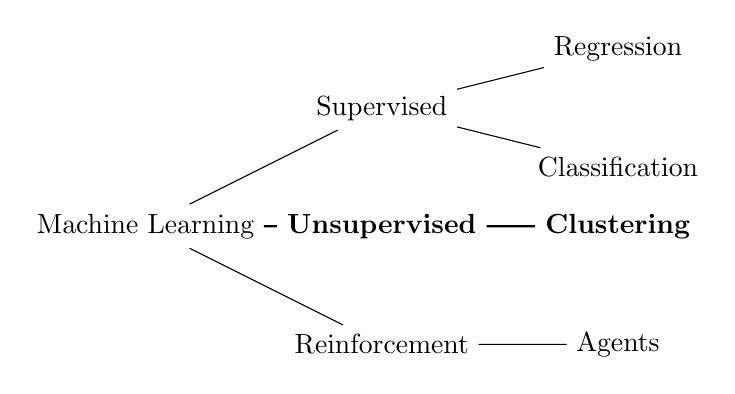
\begin{tikzpicture}[level distance=3cm]
			\node (tree) {Machine Learning} [grow'=right]
			child {node {Supervised}
				child {node {Regression}}
				child {node {Classification}}}
			child [thick] {node {\textbf{Unsupervised}}
				child {node {\textbf{Clustering}}}}
			child {node {Reinforcement}
				child {node {Agents}}};
		\end{tikzpicture}
	\end{figure}

	\begin{itemize}
		\item{Unsupervised learning: using data without
			labelled outcomes}
			\begin{itemize}
				\item{Clustering: finding clusters of data
					within dataset to discover patterns}
			\end{itemize}
	\end{itemize}
\end{frame}

\begin{frame}
	\frametitle{Types of Machine Learning Problems}

	\begin{figure}
		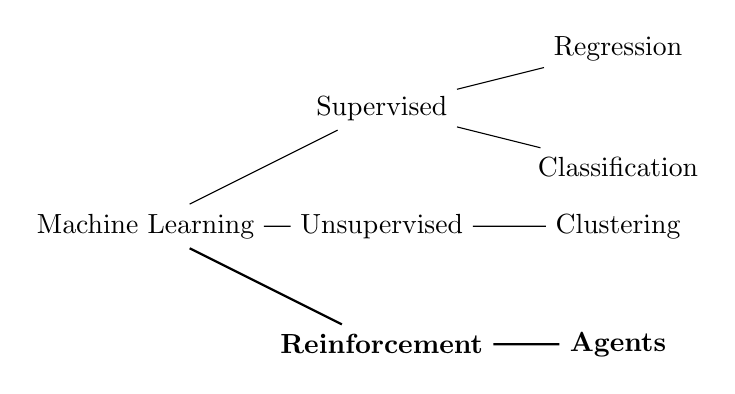
\begin{tikzpicture}[level distance=3cm]
			\node (tree) {Machine Learning} [grow'=right]
			child {node {Supervised}
				child {node {Regression}}
				child {node {Classification}}}
			child {node {Unsupervised}
				child {node {Clustering}}}
			child [thick] {node {\textbf{Reinforcement}}
				child {node {\textbf{Agents}}}};
		\end{tikzpicture}
	\end{figure}

	\begin{itemize}
		\item{Reinforcement learning: using feedback to learn a policy}
			\begin{itemize}
				\item{Agent based modelling: using
					state/environment and rewards to decide
					next action}
			\end{itemize}
	\end{itemize}
\end{frame}

\begin{frame}
	\frametitle{Machine Learning Pipeline}

	Sequential process for creating machine learning models:

	\begin{figure}
		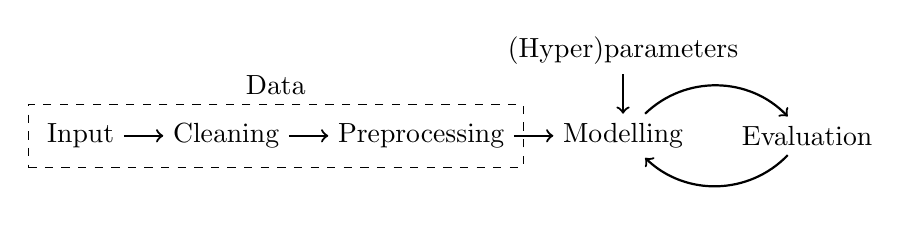
\begin{tikzpicture}[node distance=0.5cm]
			\node (input) {Input};
			\node (cleaning) [right=of input] {Cleaning};
			\node (preprocessing) [right=of cleaning]
			{Preprocessing};
			\node (modelling) [right=of preprocessing] {Modelling};
			\node (parameters) [above=of modelling] {(Hyper)parameters};
			\node (evaluation) [right=of modelling] {Evaluation};

			\node (data) [draw, dashed, label=Data, fit=(input) (cleaning)
			(preprocessing)] {};

			\draw [thick, ->] (input) -- (cleaning);
			\draw [thick, ->] (cleaning) -- (preprocessing);
			\draw [thick, ->] (preprocessing) -- (modelling);
			\draw [thick, ->] (parameters) -- (modelling);
			\draw [thick, ->]
				(modelling) edge [bend left=45] (evaluation)
				(evaluation) edge [bend left=45] (modelling);
		\end{tikzpicture}
	\end{figure}

	Significant portion dedicated to working with data -- machine learning
	techniques rely on \textbf{high quality data}!
\end{frame}

\begin{frame}
	\frametitle{Working with Data - Input}

	Multiple \textit{types} of data:

	\begin{table}
		\begin{tabular}{|l|p{5cm}|p{2cm}|}
			\hline
			\textbf{Type} & \textbf{Description} & \textbf{Examples}
			\\ \hline
			Structured & Data which strictly adheres to
			a model & DBs, CSV files \\ \hline
			Semi-structured & Data which doesn't adhere
			to a model & Log/JSON files \\ \hline
			Unstructured & Data without a structure & Media files
			\\ \hline
		\end{tabular}
	\end{table}

	When using different types of data, considerations need to be made as
	to how the data will be ``fed" to ML algorithm:
	
	\begin{itemize}
		\item{Structured data can be usually be used directly}
		\item{Semi/unstructured data may need to undergo extra
			processing to extract features}
	\end{itemize}
\end{frame}

\begin{frame}
	\frametitle{Working with Data - Cleaning}
	
	\begin{figure}
		
\begin{tikzpicture}
			\duck[broom]
		\end{tikzpicture}
	\end{figure}

	Fixing or removing data which is:

	\begin{itemize}
		\item{Incomplete}
		\item{Incorrect}
			\begin{itemize}
				\item{Logically - invalid data}
				\item{Syntactically - incorrect formatting}
			\end{itemize}
		\item{Duplicated}
		\item{Corrupted}
	\end{itemize}
\end{frame}

\begin{frame}
	\frametitle{Working with Data - Preprocessing}

	\begin{figure}
		
\begin{tikzpicture}
			\duck[glasses]
		\end{tikzpicture}
	\end{figure}

	\begin{itemize}
		\item{Transforming the data to manipulate it for specific needs}
			\begin{itemize}
				\item{Encoding - label or onehot for
					categorical values}
				\item{Most models only understand numerical
					values - need to convert strings,
					images, etc. to a numerical
					representation}
			\end{itemize}
		\item{Normalising data for efficiency/accuracy}
		\item{Feature extraction for selecting/extracting important
			features from the dataset}
	\end{itemize}
\end{frame}

\begin{frame}
	\frametitle{Modelling - Choosing a Model}

	\begin{figure}
		
\begin{tikzpicture}
			\duck[xshift=-60pt, signpost=A]
			\duck[xshift=60pt, signpost=B]
		\end{tikzpicture}
	\end{figure}

	The model we choose is heavily dependent on the \textit{problem we are trying
	to solve} - making a classifier is very different to learning a policy!

	\vspace{0.5cm}

	Other factors include:
	\begin{itemize}
		\item{Speed - how long does it take to train a model?}
		\item{Behaviour - how does the model work? How does this affect
			speed/accuracy/precision/etc.?}
		\item{Data - is the model suited to the data we are using?}
	\end{itemize}
\end{frame}

\begin{frame}
	\frametitle{\(k\)Nearest eighbours - Introduction}

	% tikz diagram showing points in space (some red/blue, one empty - input)

	\textit{General method}: use the \(k\) nearest "neighbours" in \(n\)
	dimensional space to calculate the class of new data.

	\vspace{0.5cm}

	Questions:
	\begin{itemize}
		\item{How to choose \(k\)?}
		\item{How to calculate distance?}
	\end{itemize}
\end{frame}

\begin{frame}
	\frametitle{\(k\) Nearest Neighbours - Calculating distance}
	
	% discuss euclidean vs manhattan distance
	% discuss weighting - points which are closer to input should count
	% more compared with points which are further away
\end{frame}

\begin{frame}
	\frametitle{\(k\) Nearest Neighbours - Selecting \(k\)}

	% discuss even vs odd k
	% discuss elbow method for choosing k
\end{frame}

\begin{frame}
	\frametitle{\(k\) Nearest Neighbours - Evaluation}

	% leave blank - will discuss at the end
\end{frame}



\end{document}
